\documentclass[preprint,11pt]{article}
%\documentclass{elsart3-1}

\usepackage{amsthm,amsmath,amssymb,amsfonts,amscd,amsbsy}%,latexsym,epsfig,subfig}
%\usepackage{graphicx,psfrag,verbatim,wasysym}
\usepackage{graphicx}
\usepackage[ruled,noline,linesnumbered]{algorithm2e}
%\usepackage{bm}
\usepackage[tight]{subfigure}
\usepackage{fullpage}
\usepackage{color}
%\usepackage{setspace}
%\usepackage[tight]{subfigure}
%\usepackage{listings}
\usepackage{enumerate}
\newcommand{\doi}[1]{\textsc{doi:} \textsf{#1}\xspace}

\DeclareGraphicsExtensions{.jpg,.png,.pdf}
\DeclareGraphicsRule{*}{mps}{*}{}

\setlength{\parindent}{0em}
\setlength{\parskip}{0em}

\DeclareGraphicsExtensions{.jpg,.png,.pdf}
\DeclareGraphicsRule{*}{mps}{*}{}
\graphicspath{{fig/}}



% bold letters
\newcommand{\bola}{\mathbf{a}}
\newcommand{\bolc}{\mathbf{c}}
\newcommand{\bolf}{\mathbf{f}}
\newcommand{\bolg}{\mathbf{g}}
\newcommand{\boll}{\mathbf{l}}
\newcommand{\bolq}{\mathbf{q}}
\newcommand{\bolp}{\mathbf{p}}
\newcommand{\bolu}{\mathbf{u}}
\newcommand{\bolv}{\mathbf{v}}
\newcommand{\bolw}{\mathbf{w}}
\newcommand{\bolz}{\mathbf{z}}

\newcommand{\bolA}{\mathbf{A}}
\newcommand{\bolB}{\mathbf{B}}
\newcommand{\bolC}{\mathbf{C}}
\newcommand{\bolD}{\mathbf{D}}
\newcommand{\bolE}{\mathbf{E}}
\newcommand{\bolF}{\mathbf{F}}
\newcommand{\bolG}{\mathbf{G}}
\newcommand{\bolH}{\mathbf{H}}
\newcommand{\bolI}{\mathbf{I}}
\newcommand{\bolJ}{\mathbf{J}}
\newcommand{\bolK}{\mathbf{K}}
\newcommand{\bolL}{\mathbf{L}}
\newcommand{\bolM}{\mathbf{M}}
\newcommand{\bolN}{\mathbf{N}}
\newcommand{\bolO}{\mathbf{O}}
\newcommand{\bolP}{\mathbf{P}}
\newcommand{\bolQ}{\mathbf{Q}}
\newcommand{\bolR}{\mathbf{R}}
\newcommand{\bolS}{\mathbf{S}}
\newcommand{\bolT}{\mathbf{T}}
\newcommand{\bolU}{\mathbf{U}}
\newcommand{\bolV}{\mathbf{V}}
\newcommand{\bolW}{\mathbf{W}}
\newcommand{\bolX}{\mathbf{X}}
\newcommand{\bolY}{\mathbf{Y}}
\newcommand{\bolZ}{\mathbf{Z}}

% bold symbols
\newcommand{\bolalpha}{\boldsymbol{\alpha}}
\newcommand{\bolbeta}{\boldsymbol{\beta}}
\newcommand{\boleta}{\boldsymbol{\eta}}
\newcommand{\bolpsi}{\boldsymbol{\psi}}

% shadowed letters
\newcommand{\PP}{\mathbb{P}}
\newcommand{\RR}{\mathbb{R}}
\newcommand{\CC}{\mathbb{C}}
\newcommand{\ZZ}{\mathbb{Z}}

% mathcal letters
\newcommand{\calA}{\mathcal{A}}
\newcommand{\calB}{\mathcal{B}}
\newcommand{\calC}{\mathcal{C}}
\newcommand{\calD}{\mathcal{D}}
\newcommand{\calE}{\mathcal{E}}
\newcommand{\calF}{\mathcal{F}}
\newcommand{\calG}{\mathcal{G}}
\newcommand{\calH}{\mathcal{H}}
\newcommand{\calI}{\mathcal{I}}
\newcommand{\calJ}{\mathcal{J}}
\newcommand{\calK}{\mathcal{K}}
\newcommand{\calL}{\mathcal{L}}
\newcommand{\calM}{\mathcal{M}}
\newcommand{\calN}{\mathcal{N}}
\newcommand{\calO}{\mathcal{O}}
\newcommand{\calP}{\mathcal{P}}
\newcommand{\calQ}{\mathcal{Q}}
\newcommand{\calR}{\mathcal{R}}
\newcommand{\calS}{\mathcal{S}}
\newcommand{\calT}{\mathcal{T}}
\newcommand{\calU}{\mathcal{U}}
\newcommand{\calV}{\mathcal{V}}
\newcommand{\calW}{\mathcal{W}}
\newcommand{\calX}{\mathcal{X}}
\newcommand{\calY}{\mathcal{Y}}
\newcommand{\calZ}{\mathcal{Z}}


% derivatives
\newcommand{\pp}[2]{\frac{\partial #1}{\partial #2}}
\newcommand{\dd}[2]{\frac{d #1}{d #2}}


% fraction shortcut
\newcommand{\f}[2]{\frac{#1}{#2}}
\newcommand{\slfrac}[2]{\left.#1\middle/#2\right.}

% common operators
\newcommand{\vvvert}{|\kern-1pt|\kern-1pt|}
\newcommand{\enorm}[1]{\vvvert #1 \vvvert}


% matrices
\newcommand{\bmat}[1]{\left(\begin{array}{#1}}
\newcommand{\emat}{\end{array}\right)} 



\newcommand{\blist}{\begin{list}{\ballrefb}{\leftmargin=2.0em}
  \setlength{\itemsep}{2pt}
  \setlength{\parskip}{0pt}}
\newcommand{\elist}{\end{list}}



% common format strings
\def\etal{{\it et al.}}
\def\ie{{\it i.e.}}
\def\eg{{\it e.g.}}


\DeclareMathOperator*{\arginf}{arg\,inf}
\DeclareMathOperator*{\argsup}{arg\,sup}
\DeclareMathOperator*{\argmax}{arg\,max}
\DeclareMathOperator*{\argmin}{arg\,min}


%\renewcommand{\theenumi}{(\alph{enumi})}
% 
%
%

\begin{document}

\begin{Large}\textbf{AER1418 Problem Set 1 Solution}\end{Large} \hfill %Due Thursday, January 21st, at 12:10pm.

\vspace{1em}

\section*{Part 1. Formulation and analysis}
\begin{enumerate}[(a)]
\item Since both the Neumann and Robin boundary conditions are natural boundary conditions, we choose for our function space
  \begin{equation*}
    \calV \equiv H^1(\Omega_{\rm annulus}).
  \end{equation*}
  We then invoke the weighted residual method to obtain
  \begin{align*}
    \int_{\Omega_{\rm annulus}} v (- \nabla \cdot (k \nabla u)) dx
    &=
    \int_{\Omega_{\rm annulus}} \nabla v \cdot k \nabla u dx
    - \int_{\Gamma_{\rm in}} v n \cdot k \nabla u ds
    - \int_{\Gamma_{\rm out}} v n \cdot k \nabla u ds
    \\
    &=
    \int_{\Omega_{\rm annulus}} \nabla v \cdot k \nabla u dx
    - \int_{\Gamma_{\rm in}} v g ds
    + \int_{\Gamma_{\rm out}} v (B_{\rm out} (u  -u_\infty)) ds;
  \end{align*}
  here we have applied the boundary conditions to obtain the second equality.
  We set $u_\infty = 0$ and obtain the following weak formulation: find $u \in \calV$ such that
  \begin{equation*}
    a(u,v) = \ell(v) \quad \forall v \in \calV,
  \end{equation*}
  where
  \begin{align*}
    a(w,v) &\equiv \int_{\Omega_{\rm annulus}} \nabla v \cdot k \nabla u dx + \int_{\Gamma_{\rm out}} B_{\rm out} v w ds, \\
    \ell(v) &\equiv \int_{\Gamma_{\rm in}} v g ds .
  \end{align*}
\item To recast the axisymmetric 2d problem as a 1d problem, we first introduce the function space
  \begin{equation*}
    \calV \equiv H^1(\Omega \equiv (r_{\rm in},r_{\rm out})).
  \end{equation*}
  We then make the following substitutions of the integrals: for $f \in \calV$,
  \begin{align*}
    \int_{\Omega_{\rm annulus}} f dx
    &= \int_{\Omega \equiv (r_{\rm in},r_{\rm out})} f(r) 2\pi r dr \\
    \int_{\Gamma_{\rm in}} f ds
    &= 2\pi r_{\rm in} f(r_{\rm in}) \\
    \int_{\Gamma_{\rm out}} f ds
    &= 2\pi r_{\rm out} f(r_{\rm out}).
  \end{align*}
  We have hence obtain the following weak formulation: find $u \in \calV$ such that
  \begin{equation*}
    a(u,v) = \ell(v) \quad \forall v \in \calV,
  \end{equation*}
  where
  \begin{align*}
    a(w,v) &\equiv \int_{\Omega} k x \dd{v}{x} \dd{u}{x} dx + B_{\rm out} r_{\rm out} v(r_{\rm out})w(r_{\rm out}) \\
    \ell(v) &\equiv  g r_{\rm in} v(r_{\rm in})   .
  \end{align*}
  (Note that we have divided through by $2\pi$ and are using $x$ as the coordinate variable.)
\item We first invoke the Poincar\'e-Friedrichs inequality for $\Omega \equiv (r_{\rm in}, r_{\rm out})$ and $\Gamma \equiv \{ r_{\rm out} \} \subset \partial \Omega$:  $\exists C_{\rm PF}$ such that 
  \begin{align*}
    \| v \|_{L^2(\Omega)}^2 \leq C_{\rm PF} (|v|^2_{H^1(\Omega)} + v(r_{\rm out})^2) \quad \forall v \in \calV \equiv H^1(\Omega). 
  \end{align*}
  It follows that
  \begin{align*}
    \| v \|_{H^1(\Omega)}^2
    &\equiv
    \| v \|_{L^2(\Omega)}^2  + | v |_{H^1(\Omega)}^2
    \leq
    C_{\rm PF} (|v|^2_{H^1(\Omega)} + v(r_{\rm out})^2) + | v |_{H^1(\Omega)}^2
    \\
    &= (1 + C_{\rm PF}) | v |^2_{H^1(\Omega)} +  C_{\rm PF} v(r_{\rm out})^2
    \\
    &= (1 + C_{\rm PF}) \int_{x = r_{\rm in}}^{r_{\rm out}} (\dd{v}{x})^2 dx +  C_{\rm PF} v(r_{\rm out})^2
    \\
    &\leq
    \frac{1 + C_{\rm PF}}{k r_{\rm in}} \int_{x = r_{\rm in}}^{r_{\rm out}} kx (\dd{v}{x})^2 dx +  \frac{ C_{\rm PF}}{B_{\rm out} r_{\rm out}}B_{\rm out} r_{\rm out} v(r_{\rm out})^2
    \\
    &\leq
    \max\{   \frac{1 + C_{\rm PF}}{k r_{\rm in}}, \frac{C_{\rm PF} }{B_{\rm out} r_{\rm out}} \} ( \int_{x = r_{\rm in}}^{r_{\rm out}} kx (\dd{v}{x})^2 dx + B_{\rm out} r_{\rm out} v(r_{\rm out})^2) \\
 &=
         \max\{  \frac{1 + C_{\rm PF}}{k r_{\rm in}}, \frac{C_{\rm PF} }{B_{\rm out} r_{\rm out}} \} a(v,v).
  \end{align*}
  Hence, the bilinear form is coercive with a coercivity constant
  \begin{equation*}
    \alpha = \left( \max\left\{ \frac{1 + C_{\rm PF}}{k r_{\rm in}}, \frac{ C_{\rm PF}}{B_{\rm out} r_{\rm out}} \right\} \right)^{-1}
    = \min\left\{ \frac{k r_{\rm in}}{1 + C_{\rm PF}}, \frac{B_{\rm out} r_{\rm out}}{C_{\rm PF}} \right\} > 0.
  \end{equation*}
\item The bilinear form is continuous because
  \begin{align*}
    a(w,v) &\equiv \int_{\Omega} kx \dd{v}{x} \dd{w}{x} dx + B_{\rm out} r_{\rm out} v(r_{\rm out}) w(r_{\rm out})
    \\
    &\leq
    k r_{\rm out} | v |_{H^1(\Omega)} | w |_{H^1(\Omega)} + B_{\rm out} r_{\rm out} C_{\rm tr}^2 \| v \|_{H^1(\Omega)} \| w \|_{H^1(\Omega)}
    \\
    &\leq
    \underbrace{ \max\{ k r_{\rm out}, B_{\rm out} r_{\rm out} C_{\rm tr}^2 \} }_{\equiv \gamma < \infty}  \| v \|_{H^1(\Omega)}\| w \|_{H^1(\Omega)},
  \end{align*}
  where the first inequality follows from the trace inequality, $|v(r_{\rm out})| \leq C_{\rm tr}\|v\|_{H^1(\Omega)}$, $\forall v \in \calV$.
\item The linear form is continuous because
  \begin{equation*}
    | \ell(v) | = |gr_{\rm in} v(r_{\rm in})| \leq \underbrace{ gr_{\rm in} C_{\rm tr} }_{\equiv c < \infty} \|v\|_{H^1(\Omega)}, 
  \end{equation*}
  where the inequality follows from the trace inequality.  We note that $\| \ell(\cdot) \|_{\calV'} \leq  gr_{\rm in} C_{\rm tr}$.
\item We note that all conditions of the Lax-Milgram theorem are satisfied: $\Omega$ is a Lipschitz domain; $a(\cdot,\cdot)$ is coercive and continuous; and $\ell(\cdot)$ is continuous.  Hence, a unique solution to the variational problem exists.
\item Let $B_{\rm out} = 0$.  Then, for $v = 1 \in H^1(\Omega)$,
  \begin{equation*}
    a(v,v) = \int_{\Omega} k x \dd{v}{x} \dd{v}{x} dx = \int_{\Omega} k x 0 dx = 0.
  \end{equation*}
  Since $\| v \|_{H^1(\Omega)}^2 = | 1 |_{H^1(\Omega)}^2 + \int_{r_{\rm in}}^{r_{\rm out}} 1^2 dx = r_{\rm out} - r_{\rm in} > 0 $, we conclude that there is no $\alpha > 0$ for which $a(v,v) \geq \alpha \| v \|_{H^1(\Omega)}^2$; hence, the bilinear form is not coercive.

  The problem does not have a unique solution.  In particular, suppose $u \in \calV$ is a solution to the variational form.  Then, $u + c$, where $c$ is any constant function, is also a solution to the variational form because $a(u+c,v) = a(u,v) = \ell(v)$ $\forall v \in \calV$.
\item We recognize the bilinear form identified in (b) is symmetric and coercive.  Hence, the minimization form of the variational problem is as follows: find $u \in \calV \equiv H^1(\Omega)$ such that
  \begin{align*}
    u = \argmin_{w \in \calV} J(w),
  \end{align*}
  where
  \begin{align*}
    J(w) \equiv \frac{1}{2} a(w,w) - \ell(w)
    =
    \frac{1}{2} \int_{\Omega} k x \dd{w}{x} \dd{u}{x} dx + B_{\rm out} r_{\rm out} w(r_{\rm out})w(r_{\rm out}) 
    -  g r_{\rm in} w(r_{\rm in})   .
  \end{align*}
\end{enumerate}


\section*{Part 2. Implementation}
\begin{enumerate}
\item To discretize the problem, we first introduce nodes $r_{\rm in} \equiv x_1 < x_2 < \cdots < x_n \equiv r_{\rm out}$.  For an element $K_i$ on $(x_i,x_{i+1})$, the local contribution to the stiffness matrix from the volume terms are
  \begin{align*}
     \int_{K_i} kx \dd{\phi_i}{x} \dd{\phi_i}{x} dx
     &= \int_{x_i}^{x_{i+1}} k x (-\frac{1}{h_i})^2 dx
     = k \frac{1}{2} ( x_{i+1}^2 - x_i^2 ) \frac{1}{h_i^2}
     = k \frac{1}{2} (x_{i+1} + x_i) \frac{1}{h_i}
     = k x^{K_i}_c \frac{1}{h_i}
     \\
     \int_{K_i} kx \dd{\phi_{i+1}}{x} \dd{\phi_{i+1}}{x} dx
     &= \int_{x_i}^{x_{i+1}} k x (\frac{1}{h_i})^2 dx
     = k x^{K_i}_c \frac{1}{h_i}
     \\
     \int_{K_i} kx \dd{\phi_i}{x} \dd{\phi_{i+1}}{x} dx
     &= \int_{x_i}^{x_{i+1}} k x (-\frac{1}{h_i})(\frac{1}{h_i}) dx
     = - k \frac{1}{2} ( x_{i+1}^2 - x_i^2 ) \frac{1}{h_i^2}
     = - k x_c^{K_i} \frac{1}{h_i},
  \end{align*}
  where $h_{i} \equiv x_{i+1} - x_i$ and $x^{K_i}_c \equiv \frac{1}{2} (x_{i+1} + x_i)$. The Robin boundary contribution to the stiffness matrix is
  \begin{equation*}
    B_{\rm out} r_{\rm out} [\phi_i \phi_i]_{x = r_{\rm out}} = \begin{cases}
      B_{\rm out} r_{\rm out}, \quad i = n, \\
      0 , \quad \text{otherwise}.
    \end{cases}
  \end{equation*}
  The Neumann boundary contribution to the load vector is
  \begin{equation*}
    g r_{\rm in} [\phi_i ]_{x = r_{\rm in}} = \begin{cases}
      g r_{\rm in}, \quad i = 1, \\
      0 , \quad \text{otherwise}.
    \end{cases}
  \end{equation*}
  Putting everything together, the entries of the stiffness matrix are given by
  \begin{align*}
    a(\phi_1,\phi_1) &= \int_\Omega kx \dd{\phi_1}{x}  \dd{\phi_1}{x} dx = kx_c^{K_1} \frac{1}{h_1}, \\
    a(\phi_i,\phi_i) &= \int_\Omega kx \dd{\phi_i}{x}\dd{\phi_i}{x} dx =  kx_c^{K_{i-1}} \frac{1}{h_{i-1}} + kx_c^{K_i} \frac{1}{h_i}, \quad i = 2, \dots, n-1, \\
    a(\phi_n,\phi_n) &= \int_\Omega kx \dd{\phi_n}{x}\dd{\phi_n}{x} dx = kx_c^{K_{n-1}} \frac{1}{h_{n-1}}, \\
    a(\phi_i,\phi_{i+1}) &= a(\phi_{i+1},\phi_i) =\int_\Omega kx \dd{\phi_i}{x} \dd{\phi_{i+1}}{x} dx = -k x_c^{K_i} \frac{1}{h_i}, \quad i = 1,\dots, n-1.
  \end{align*}
  The load vector is given by
  \begin{align*}
    \ell(\phi_1) &= g r_{\rm in}, \\
    \ell(\phi_i) &= 0, \quad i = 2,\dots, n.
  \end{align*}
\item The finite element solution for for $r_{\rm in} = 1/2$, $r_{\rm out} = 2$, $k = 1$, $g = 1$, $B_{\rm out} = 1$, and $h = 1/4$ is shown in Figure~\ref{fig:state}.
  \begin{figure}[!h]
    \centering
    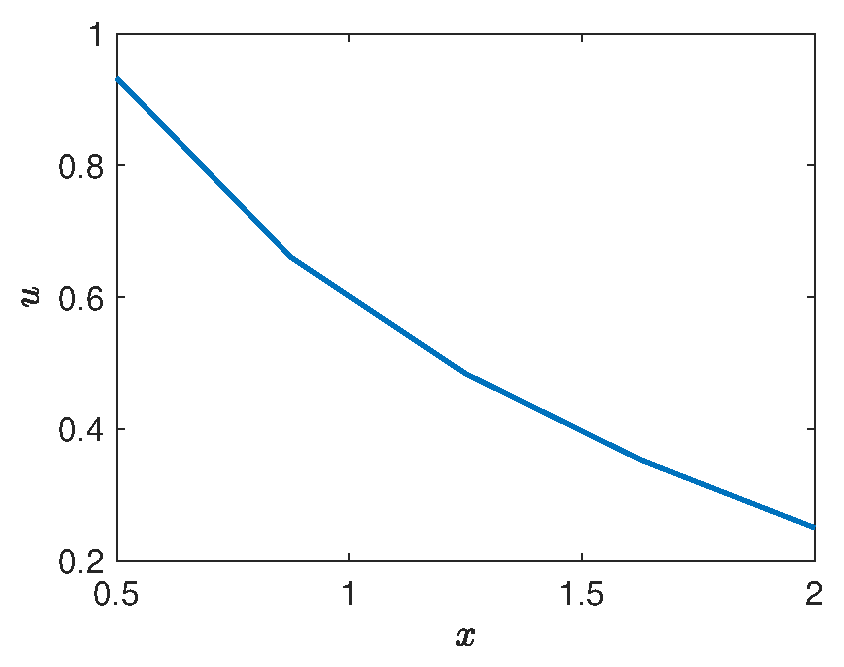
\includegraphics[width=0.45\textwidth]{state}
    \caption{Solution field. \label{fig:state}}
  \end{figure}
\item We note that $\ell^o(w) \equiv gr_{\rm in} w(r_{\rm in}) = \ell(w)$, $\forall w \in \calV$. It hence follows
  \begin{align*}
    \ell^o(u) - \ell^o(u_h)
    &= \ell(u) - \ell(u_h) & \text{(equivalence of $\ell$ and $\ell^o$)} \\
    &= \ell(u - u_h) & \text{(linearity of $\ell$)} \\
    &= a(u, u - u_h) & \text{($a(u,v) = \ell(v)$, $\forall v \in \calV$)} \\
    &= a(u - u_h, u - u_h), & \text{(Galerkin orthogonality)}
  \end{align*}
  which is the desired equality.
\item
  The reference output computed is
  \begin{equation*}
    \ell^o(u_{h_{\rm ref}}) \approx 0.47157344.
  \end{equation*}
  The convergence plot for the output is shown in Figure~\ref{fig:conv}.  The error varies as $e \sim h^r$ and hence produces a line in log-log scale.
  \begin{figure}[!h]
    \centering
    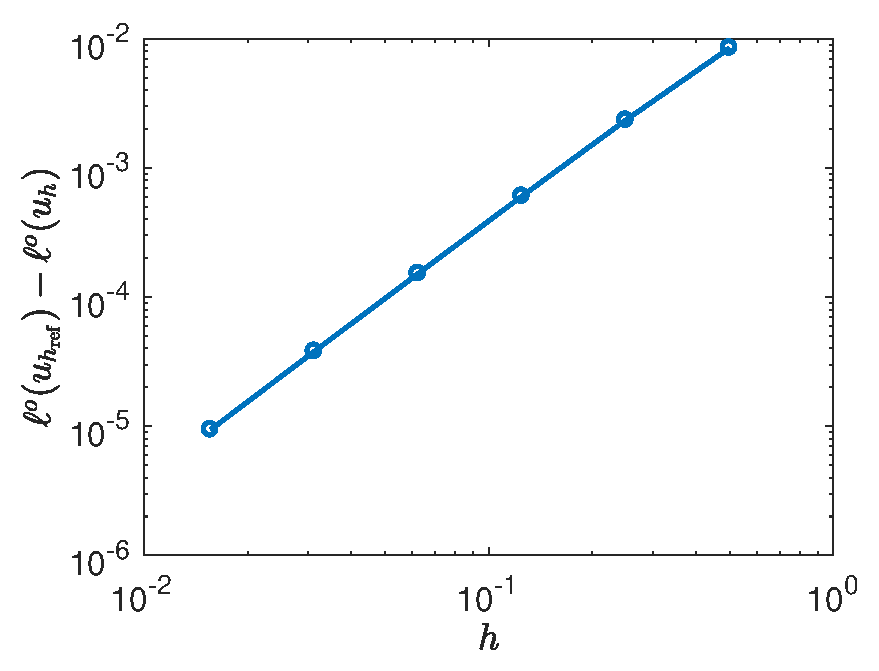
\includegraphics[width=0.45\textwidth]{conv}
    \caption{Output convergence. \label{fig:conv}}
  \end{figure}
  The observed convergence rate for the two finest meshes is
  \begin{equation*}
    r_{\rm obs} = \frac{\log(\ell^o(u_{h = 1/64}) / \ell^o(u_{h = 1/32}))}{ \log( (1/64) / (1/32))} \approx 2.016.
  \end{equation*}
  We recall that the energy norm of the error converges as $\enorm{e} \equiv \sqrt{a(e,e)} \leq C \max_{x \in \Omega} | e'' | h$ for the linear finite element approximation of a smooth solution.  We hence expect, for the smooth solution, the output error $|\ell^o(e)| = |a(e,e)|$ to converge as $\sim h^2$, the \emph{square} of the energy norm of the error.  The observed rate of 2.016 is close to the theoretical rate of 2.
\end{enumerate}

\end{document}

